\chapter{結果}
\label{chap:結果}

\section{RenderBoxの評価}
\label{sec:RenderBoxの評価}

\begin{table}[htbp]
\centering
\caption{RenderBox \cite{RenderBox} との性能比較（括弧内は文献値）}
\label{tab:renderbox_evaluation}
\resizebox{\textwidth}{!}{%
\begin{tabular}{lcccc} % {lcccc{6cm}} から {lcccc} に修正（5列）
\toprule
\textbf{Model} & \textbf{FAD} $\downarrow$ & \textbf{Pitch} $\uparrow$ & \textbf{Tempo} $\downarrow$ & \textbf{CLAP} $\uparrow$ \\ 
\midrule
% --- Stage 0 (w/o align) ---
Stage 0 & 61.8793 & 0.792 & 16.89 & 0.071 \\
 & (839.3) & (0.794) & (0.038) & (0.174) \\ 
\midrule
% --- Stage 2 ---
Stage 2 & 96.2042 & 0.8130 & 18.55 & 0.069 \\
 & (562.58) & (0.753) & (10.39) & (0.265) \\ 
\midrule
% --- Stage 4 ---
Stage 4 & 74.7507 & 0.8093 & 16.00 & 0.068 \\
 & (340.77) & (0.748) & (19.51) & (0.234) \\ % 末尾の余計な & を削除
\bottomrule
\end{tabular}
}
\end{table}

\begin{figure}[htbp]
    \centering
    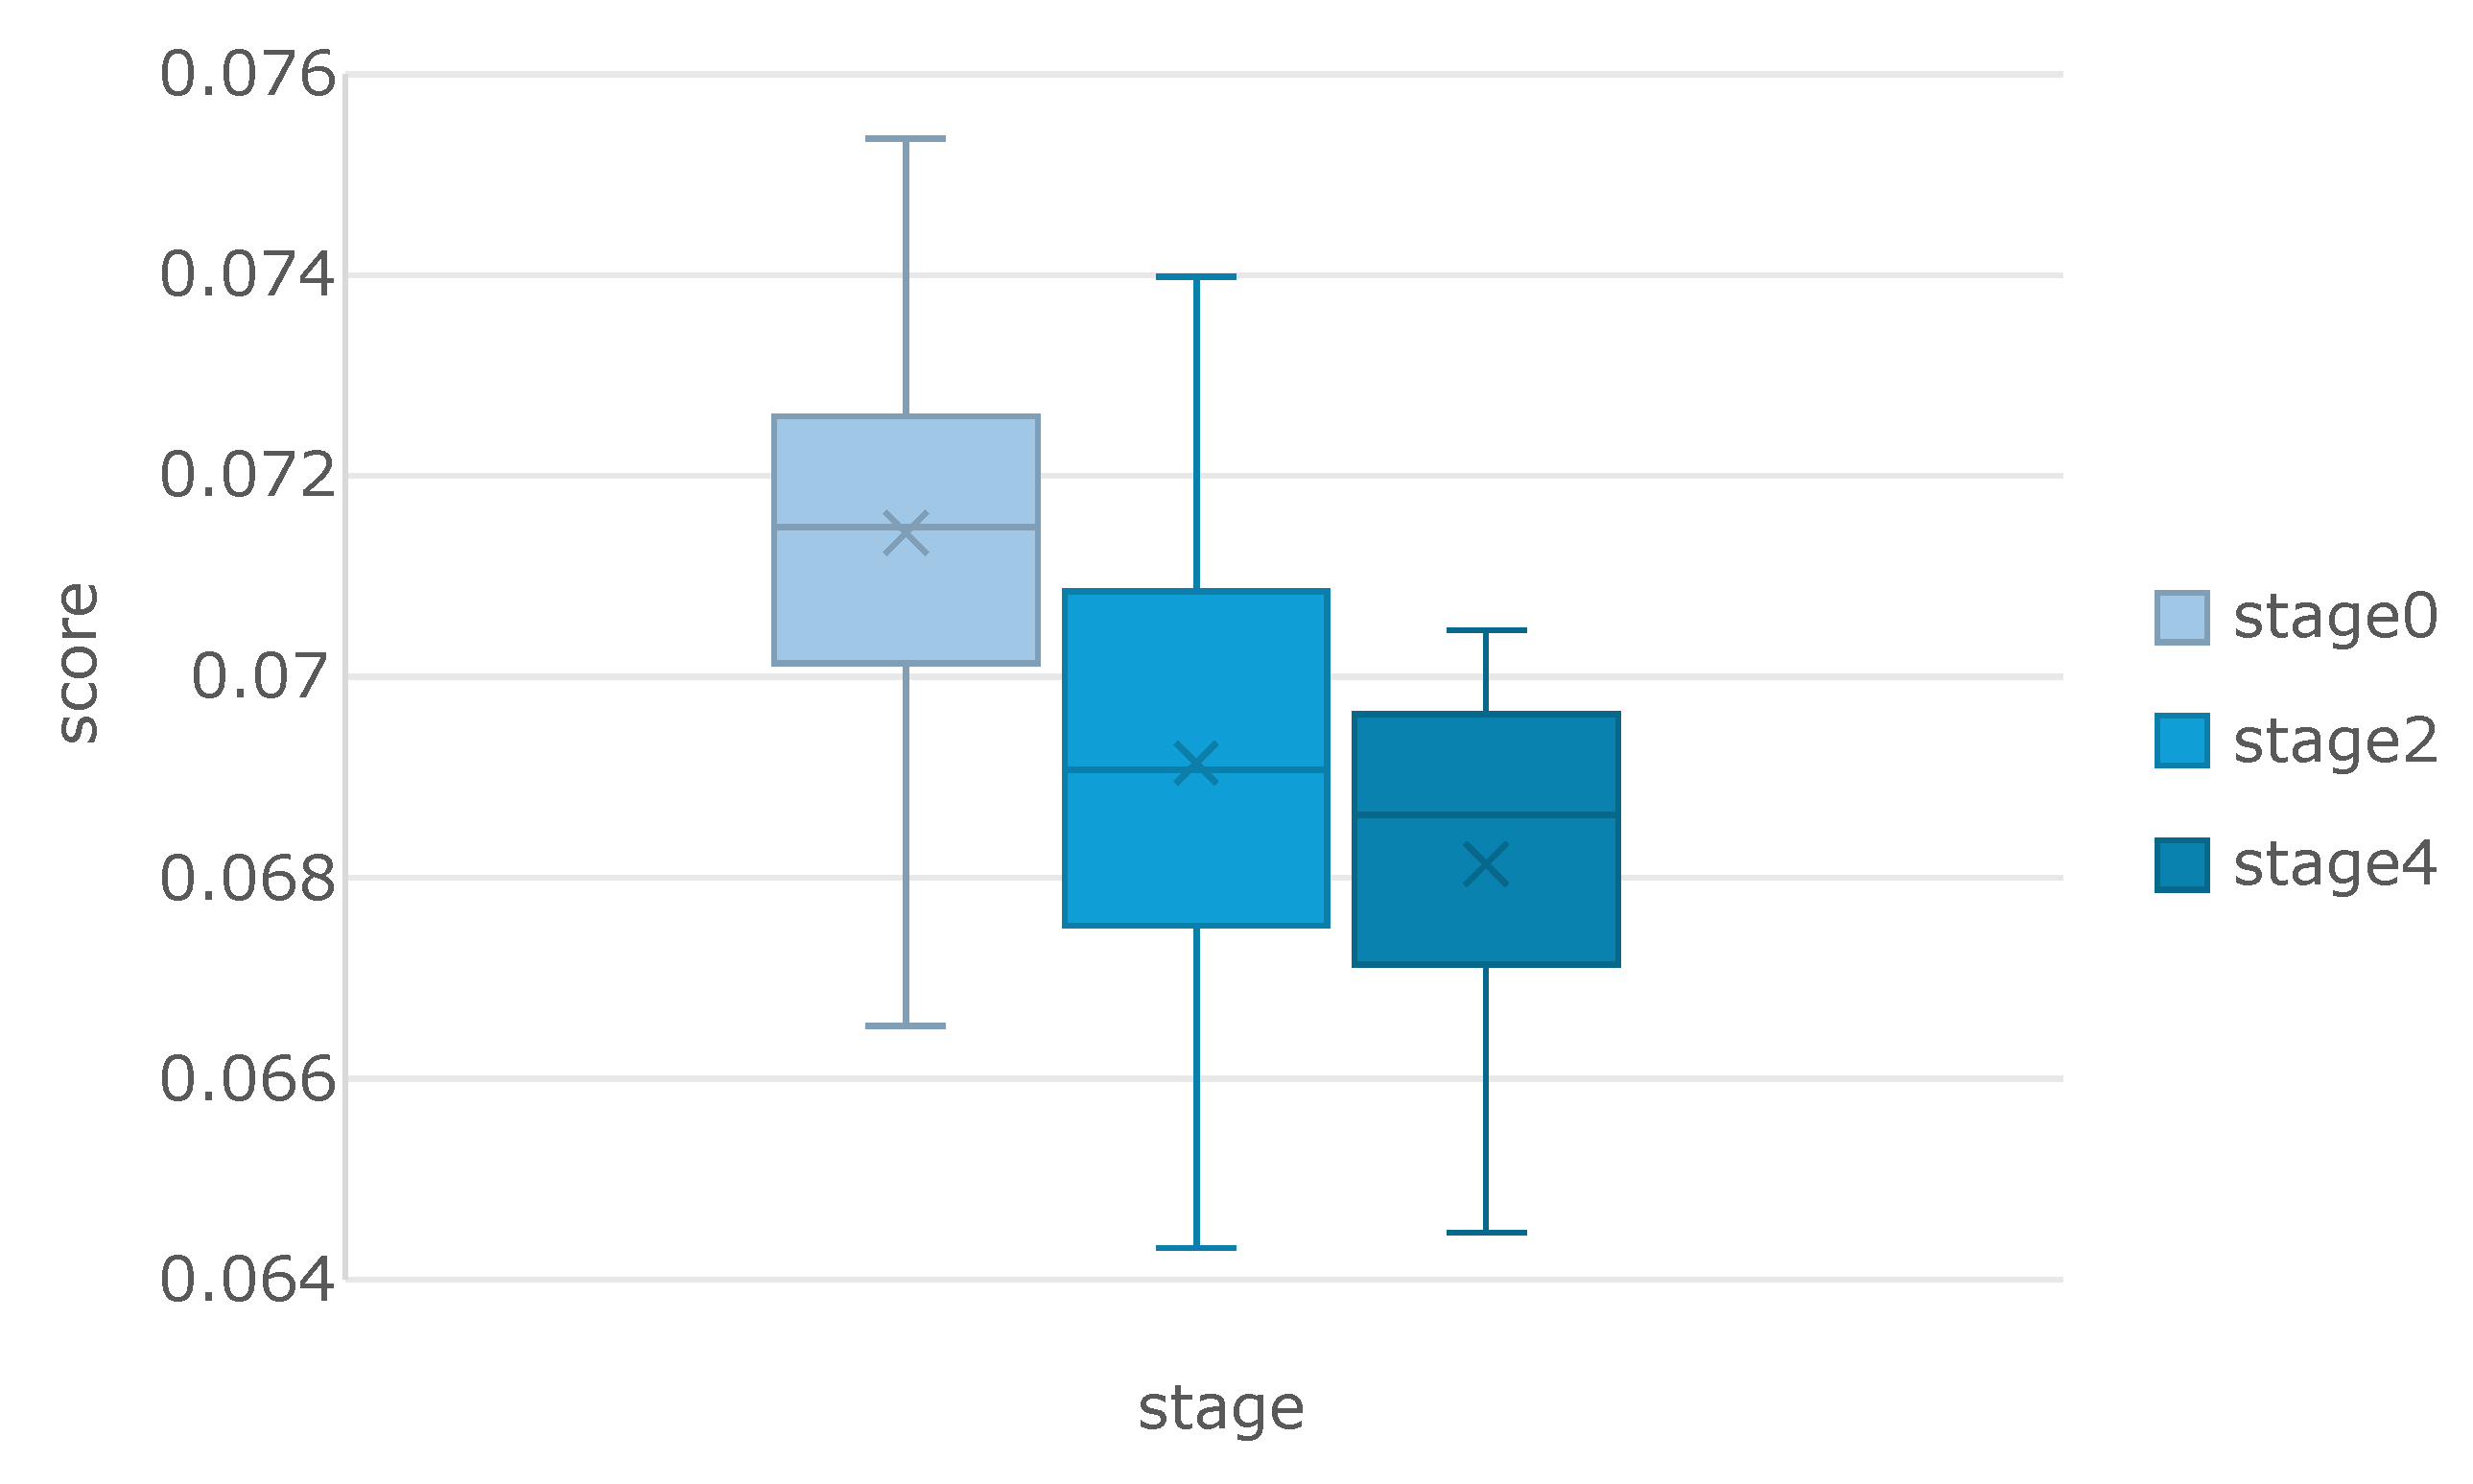
\includegraphics[width=1.0\linewidth]{figs/5/clap.pdf}
    \caption{RenderBoxの性能評価：CLAP score}
    \label{fig:RenderBox_CLAP}
\end{figure}

\begin{figure}[htbp]
    \centering
    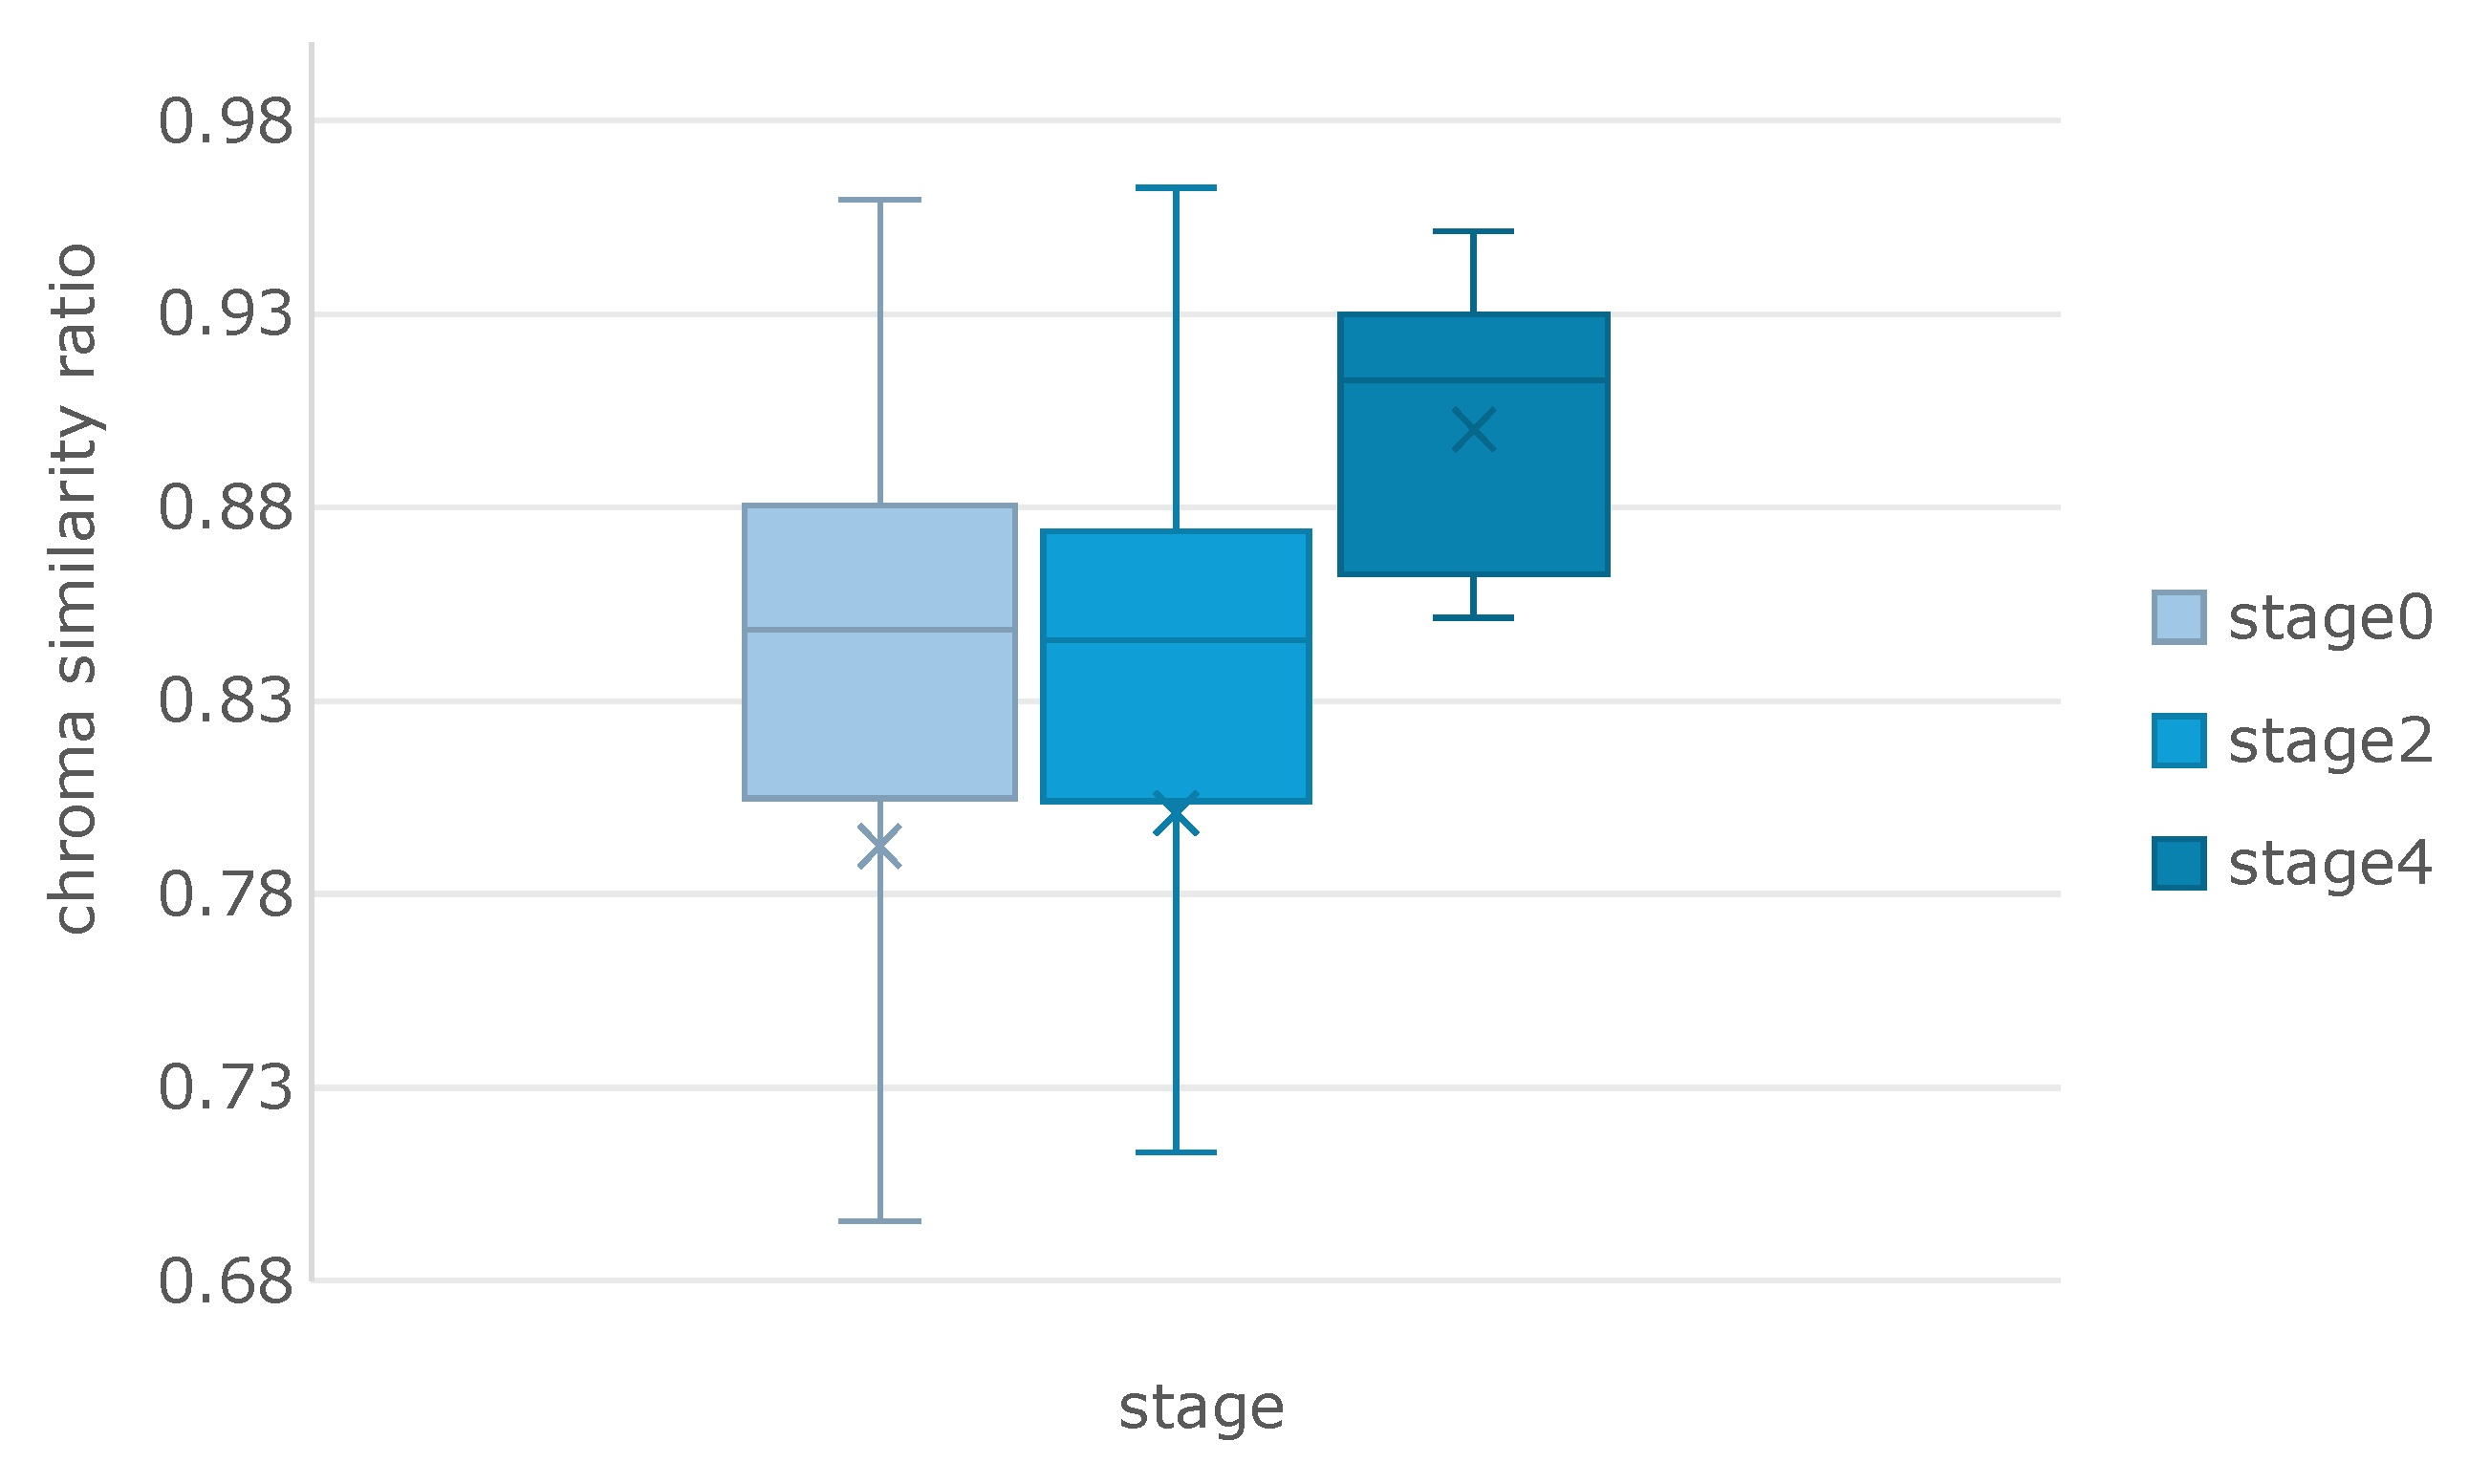
\includegraphics[width=1.0\linewidth]{figs/5/Pitch.pdf}
    \caption{RenderBoxの性能評価：pitchの正確さ}
    \label{fig:RenderBox_pitch}
\end{figure}

\begin{figure}[htbp]
    \centering
    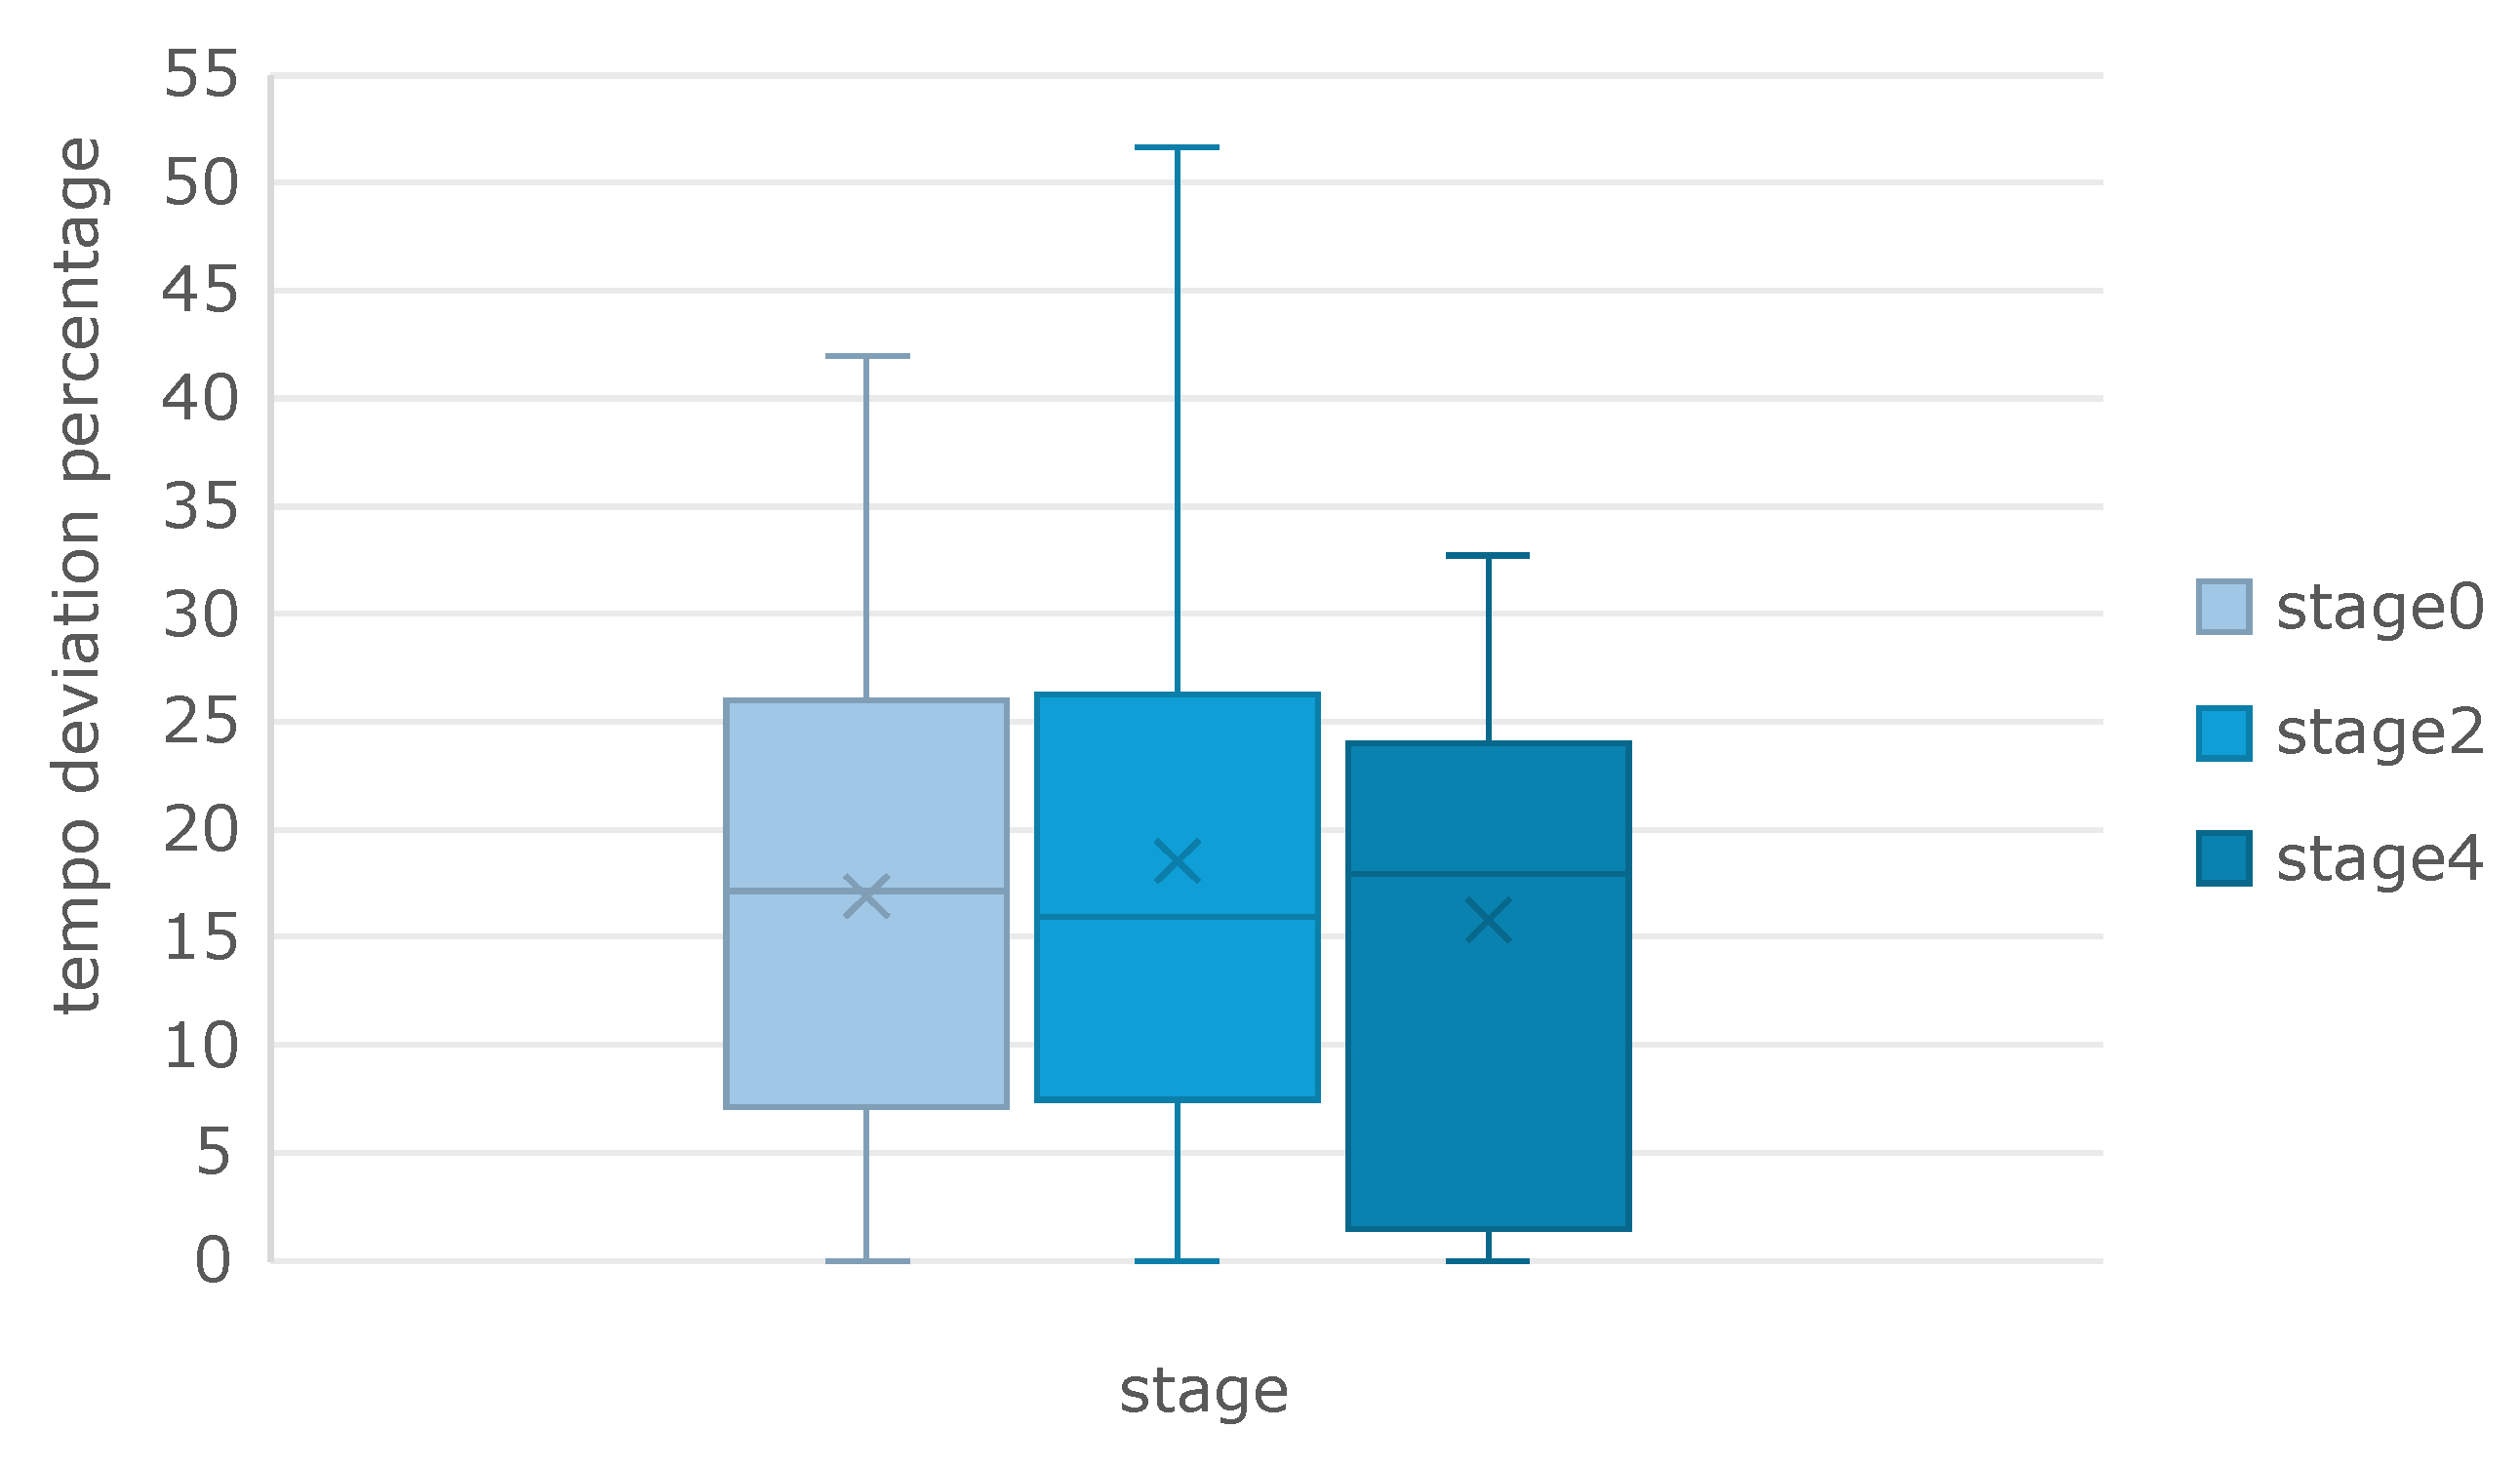
\includegraphics[width=1.0\linewidth]{figs/5/tempo_deviation.pdf}
    \caption{RenderBoxの性能評価：tempoのずれ} % temo -> tempo に修正
    \label{fig:RenderBox_tempo}
\end{figure}

\section{提案システムの評価}
\label{sec:提案システムの評価}

\subsection{客観評価}
\label{subsec:客観評価}
% ここに本文を記述

\subsection{主観評価}
\label{subsec:主観評価}
% ここに本文を記述